\documentclass[25pt, portrait, a1paper]{tikzposter}
\usepackage{tikz}
\usepackage{adjustbox}
\usepackage{textcomp}
\usepackage{multicol}
\usepackage{amsmath}
% \usepackage{amssymb}
\usetikzlibrary{shapes, arrows.meta}
\usetheme{Default}

\begin{document}

%   \begin{columns}
%     \column{0.5}
  \block[titleoffsety=.49\textheight, bodyoffsety=.49\textheight, bodywidthscale=1.04, titlewidthscale=1.04]{More details on the GLO model}{
	\begin{center}
% 	  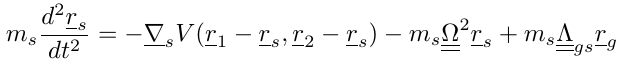
\includegraphics[width = .8\textwidth]{abb/GLO_eq1.png}
	  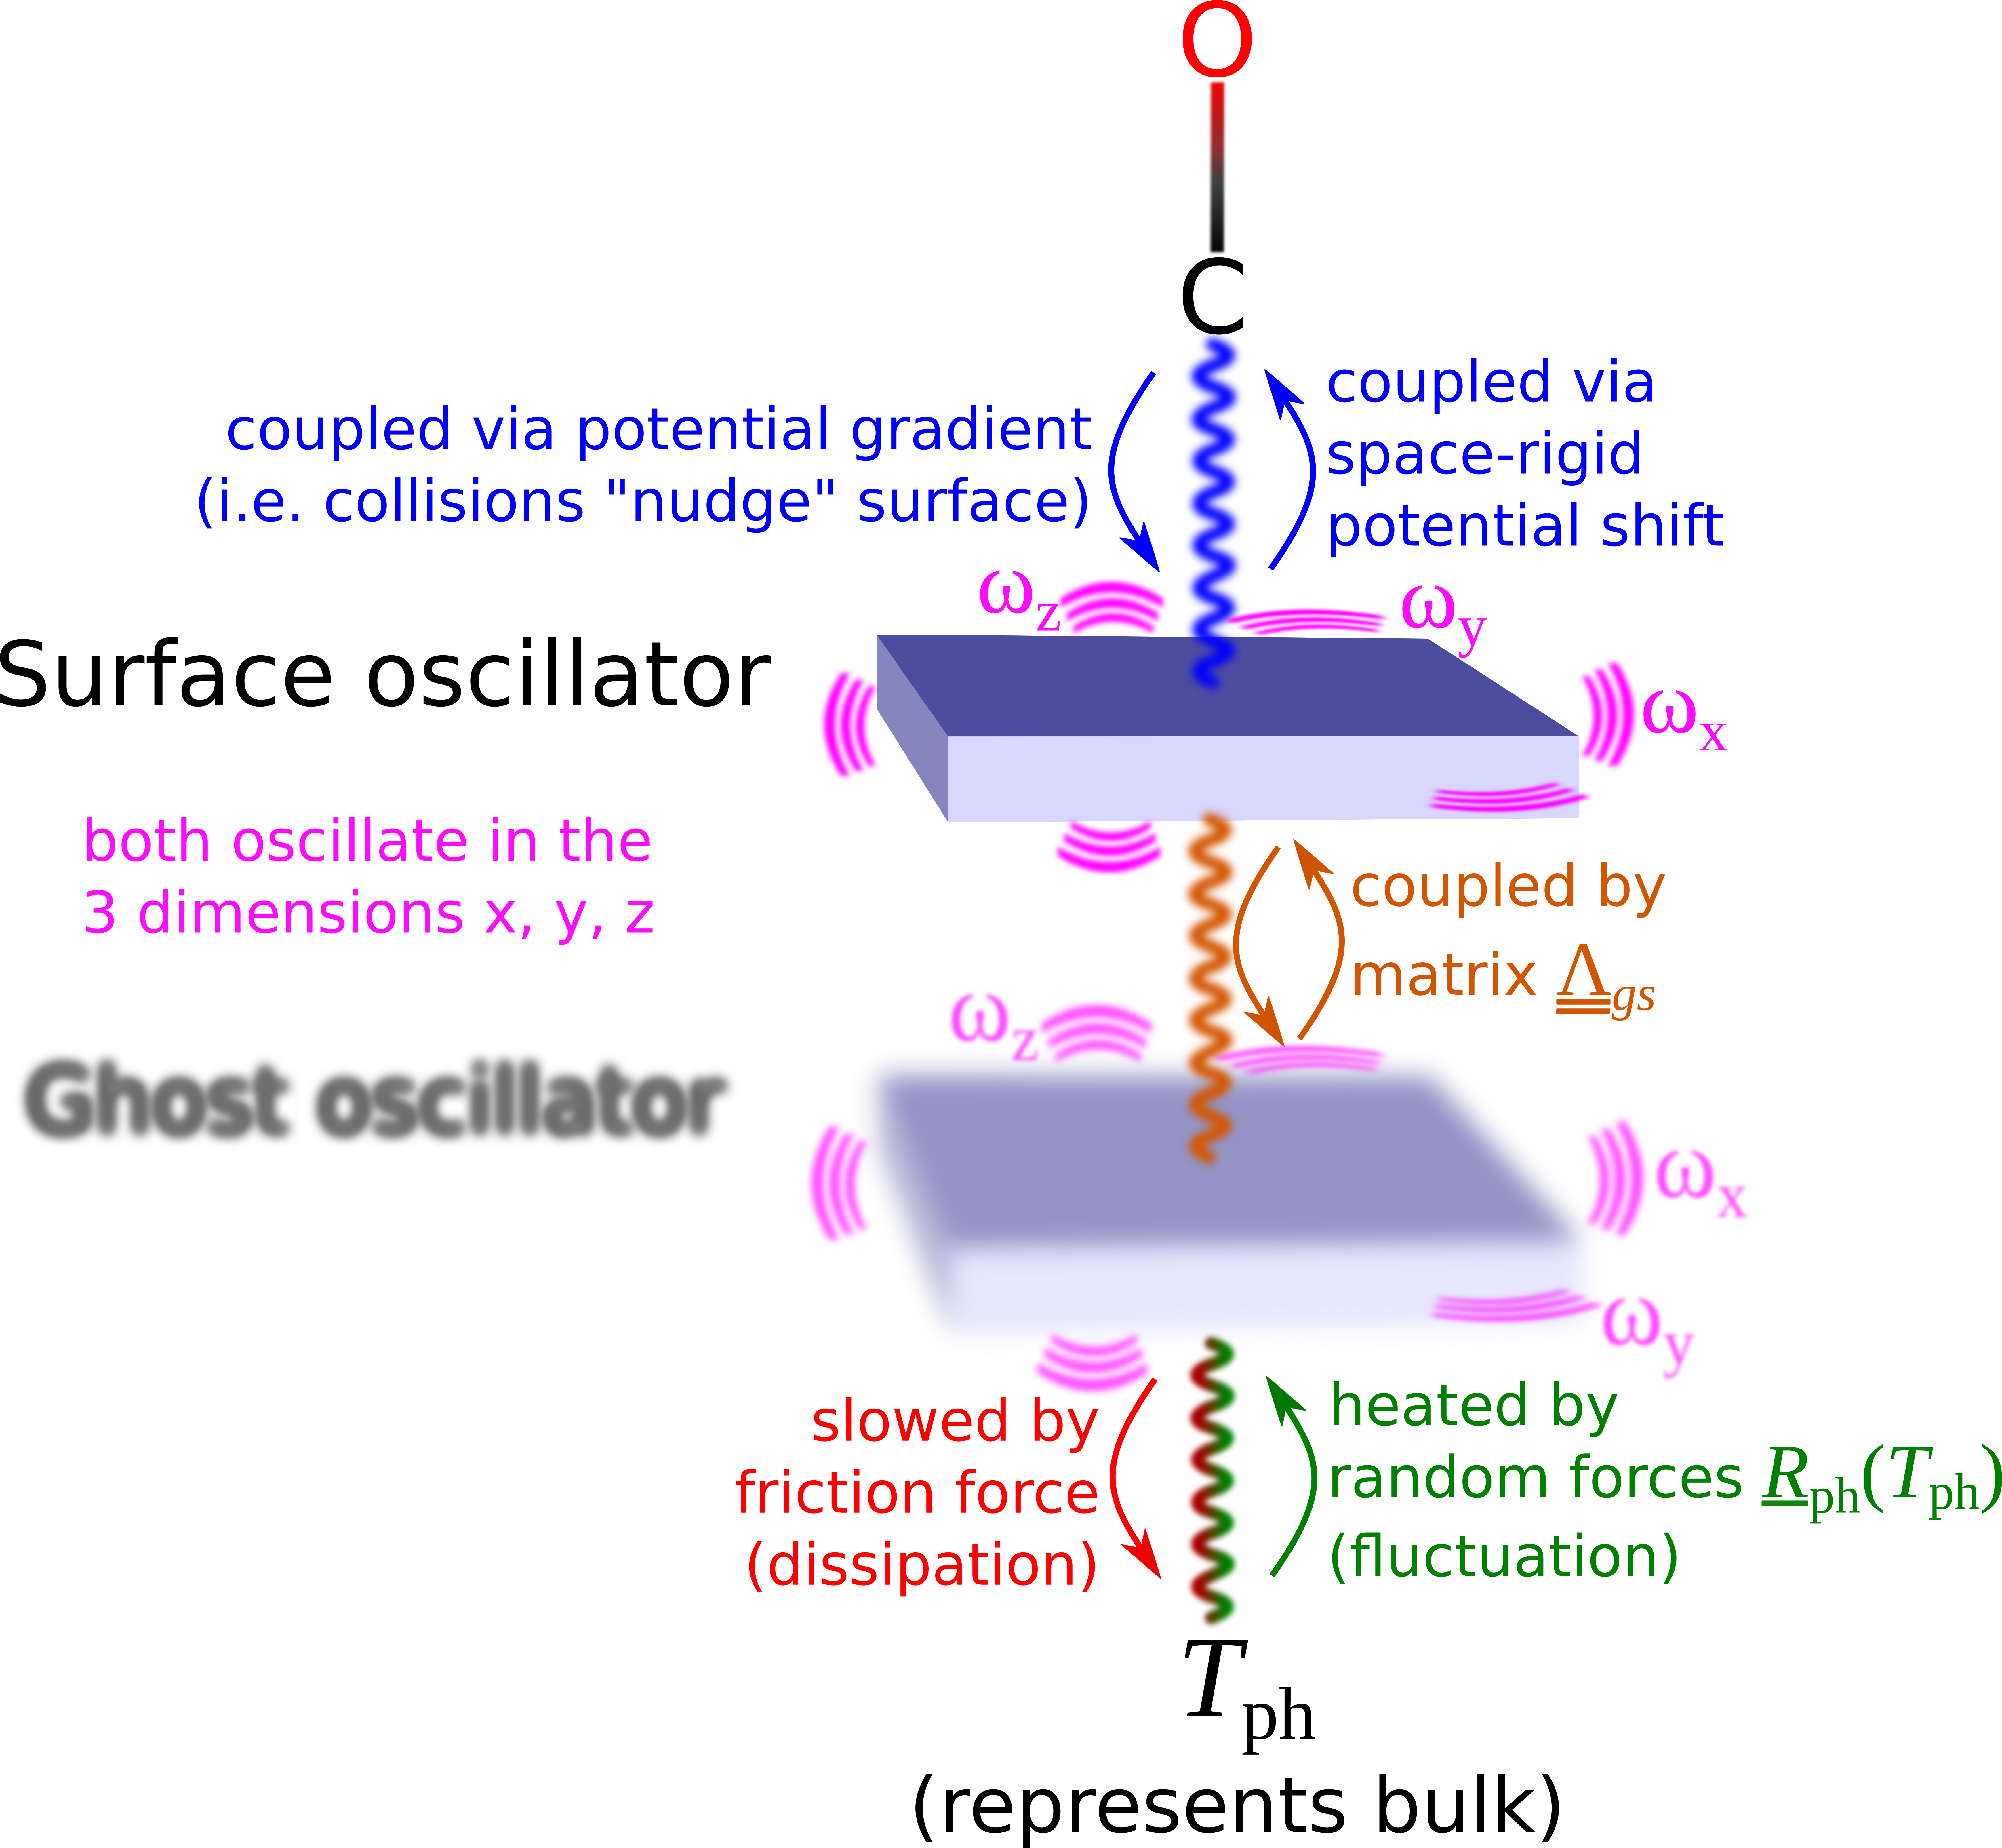
\includegraphics[width = .75\textwidth]{abb/GLO.png}
	  \begin{itemize}\huge
	  	\item Equations of motion for surface oscillator $\underline{r}_s$ and ghost oscillator $\underline{r}_g$: 
	  \end{itemize}
	  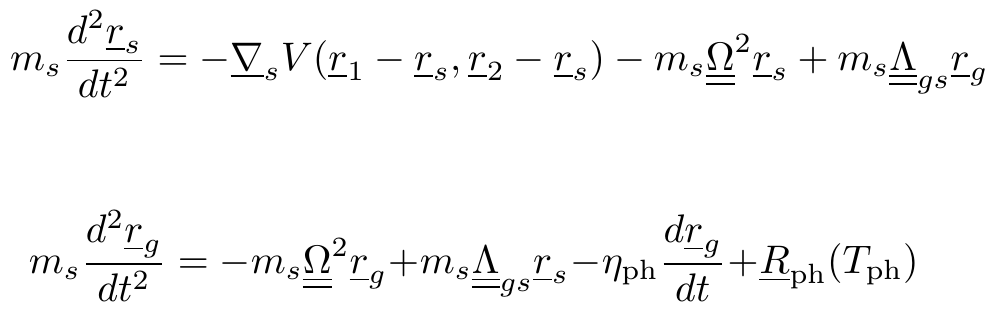
\includegraphics[width = .7\textwidth]{abb/GLO_eqs.png}
  \end{center}
  }
%   \block[bodywidthscale=0.1]{}{}
  \block{Contact information Robert Scholz:}{
	\textbf{Adress:} 
	Haus 25, Raum D2.04/05, 
	Institut f\"ur Chemie, 
	Universit\"at Potsdam, 
	Karl-Liebknecht-Str. 24-25, 
	D-14476 Potsdam\\
	\textbf{Tel.:} 0331-977-5368\\	
	\textbf{Email:} roscholz@uni-potsdam.de
  }
%     \column{0.5}    
%   \end{columns}
\end{document}
